\documentclass[tikz,border=8pt]{standalone}
% Shared look for every TikZ diagram. Load with \input{../../tools/tikz-style.tex}
\usepackage[T1]{fontenc}
\usepackage{lmodern}
\renewcommand{\sfdefault}{lmr}  % diagrams use the same serif as the text
\usetikzlibrary{arrows.meta, positioning, shapes.geometric, calc, fit, backgrounds}
\definecolor{cblue}{HTML}{4C78A8}
\definecolor{corange}{HTML}{F58518}
\definecolor{cgreen}{HTML}{54A24B}
\definecolor{cred}{HTML}{E45756}
\definecolor{cpurple}{HTML}{B279A2}
\definecolor{cgrey}{HTML}{6B6B6B}
\tikzset{
  every picture/.style={font=\sffamily, line width=1.2pt},
  box/.style={draw=#1, fill=#1!12, rounded corners=4pt, align=center, inner sep=7pt, minimum height=1.1cm},
  box/.default=cgrey,
  arrow/.style={-{Stealth[length=3mm]}, draw=cgrey, line width=1.4pt},
  title/.style={font=\sffamily\bfseries\Large},
  note/.style={font=\sffamily\small, text=cgrey, align=center},
}
\AtBeginDocument{\hyphenpenalty=10000 \exhyphenpenalty=10000}

\begin{document}
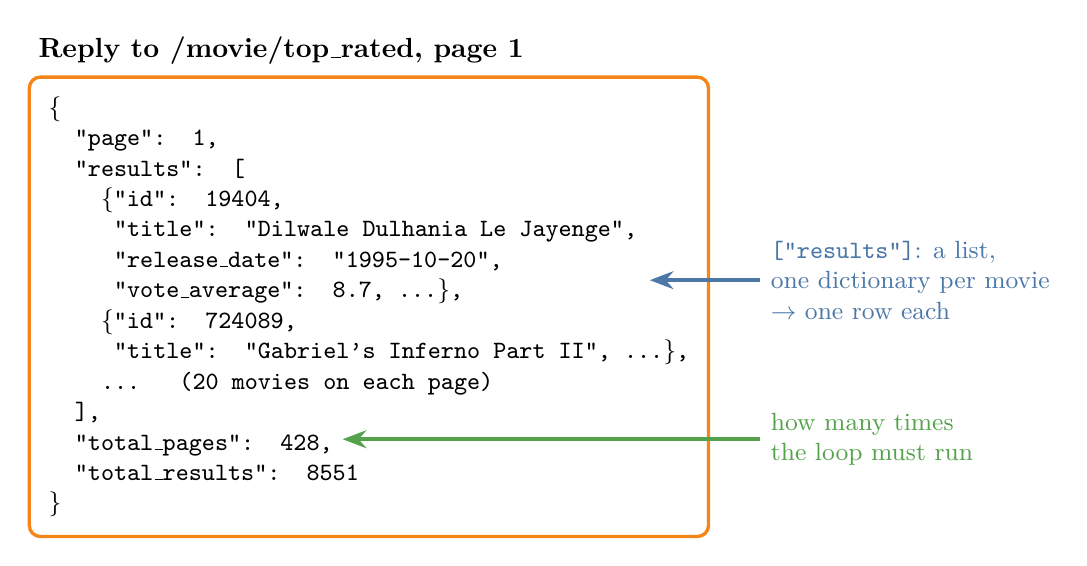
\begin{tikzpicture}
  \node[box=corange, fill=white, align=left, font=\ttfamily\small, anchor=north west] (j) at (0,0) {%
\{\\
\ \ "page": 1,\\
\ \ "results": [\\
\ \ \ \ \{"id": 19404,\\
\ \ \ \ \ "title": "Dilwale Dulhania Le Jayenge",\\
\ \ \ \ \ "release\_date": "1995-10-20",\\
\ \ \ \ \ "vote\_average": 8.7, ...\},\\
\ \ \ \ \{"id": 724089,\\
\ \ \ \ \ "title": "Gabriel's Inferno Part II", ...\},\\
\ \ \ \ ...\ \ \ (20 movies on each page)\\
\ \ ],\\
\ \ "total\_pages": 428,\\
\ \ "total\_results": 8551\\
\}};
  \node[anchor=south west, font=\sffamily\bfseries] at (j.north west) {Reply to /movie/top\_rated, page 1};
  % callouts
  \node[note, anchor=west, text=cblue, align=left] (c1) at (9.3,-2.6) {\texttt{["results"]}: a list,\\one dictionary per movie\\$\rightarrow$ one row each};
  \draw[arrow, draw=cblue] (c1.west) -- (7.9,-2.6);
  \node[note, anchor=west, text=cgreen, align=left] (c2) at (9.3,-4.62) {how many times\\the loop must run};
  \draw[arrow, draw=cgreen] (c2.west) -- (4.0,-4.62);
\end{tikzpicture}
\end{document}
